% \iffalse meta-comment
%
% Copyright (C) 2009 by Dangerous Curve <typesetting@dangerouscurve.org>
% -------------------------------------------------------
% 
% This file may be distributed and/or modified under the
% conditions of the LaTeX Project Public License, either version 1.2
% of this license or (at your option) any later version.
% The latest version of this license is in:
%
%    http://www.latex-project.org/lppl.txt
%
% and version 1.2 or later is part of all distributions of LaTeX 
% version 1999/12/01 or later.
%
% \fi
%
% \iffalse
%<*driver>
\ProvidesFile{admbmanual.dtx}
%</driver>
%<class>\NeedsTeXFormat{LaTeX2e}[1999/12/01]
%<class>\ProvidesClass{admbmanual}
%<*class>
    [2009/06/01 v1.0 ADMBMANUAL class file]
%</class>
%
%<*driver>
\documentclass{ltxdoc}
\EnableCrossrefs         
\CodelineIndex
\RecordChanges
%\OnlyDescription
\begin{document}
  \DocInput{admbmanual.dtx}
\end{document}
%</driver>
% \fi
%
% \CheckSum{0}
%
% \CharacterTable
%  {Upper-case    \A\B\C\D\E\F\G\H\I\J\K\L\M\N\O\P\Q\R\S\T\U\V\W\X\Y\Z
%   Lower-case    \a\b\c\d\e\f\g\h\i\j\k\l\m\n\o\p\q\r\s\t\u\v\w\x\y\z
%   Digits        \0\1\2\3\4\5\6\7\8\9
%   Exclamation   \!     Double quote  \"     Hash (number) \#
%   Dollar        \$     Percent       \%     Ampersand     \&
%   Acute accent  \'     Left paren    \(     Right paren   \)
%   Asterisk      \*     Plus          \+     Comma         \,
%   Minus         \-     Point         \.     Solidus       \/
%   Colon         \:     Semicolon     \;     Less than     \<
%   Equals        \=     Greater than  \>     Question mark \?
%   Commercial at \@     Left bracket  \[     Backslash     \\
%   Right bracket \]     Circumflex    \^     Underscore    \_
%   Grave accent  \`     Left brace    \{     Vertical bar  \|
%   Right brace   \}     Tilde         \~}

%
% \changes{v1.0}{2009/06/01}{Initial version}
%
% \GetFileInfo{admbmanual.dtx}
%
% \DoNotIndex{\newcommand,\newenvironment}
% \DoNotIndex{\#,\$,\%,\&,\@,\\,\{,\},\^,\_,\~,\ } 
% \DoNotIndex{\@ne} 
% \DoNotIndex{\advance,\begingroup,\catcode,\closein} 
% \DoNotIndex{\closeout,\day,\def,\edef,\else,\empty,\endgroup} 
% 
%
% \title{The \textsf{admbmanual} class\thanks{This document
%   corresponds to \textsf{admbmanual}~\fileversion, dated \filedate.}}
% \author{Dangerous Curve\\ \texttt{typesetting@dangerouscurve.org}}
%
% \maketitle
%
% \section{Introduction}
%
% The admbmanual class lets you write manuals in the style of the \textsc{admb} Project.
%
%
% \section{Usage for the Manual Writer}
%
% \subsection{Get Started with a Sample Skeleton}
%
% You can use the file |admb-sample.tex|, which contains a simple skeleton example, as the starting point for your manual.
%
% To compile your manual, you need to use the Makefile by running the command |make| on the command line.  If your \LaTeX's file name is |admb-sample.tex|, then type: |make filename=admb-sample|
%
% If you want to clear out intermediate auxiliary files left around by \LaTeX, type (again, for |admb-sample.tex|): |make clean filename=admb-sample|
%
%
% \subsection{Use Standard \LaTeX}
%
% Insofar as we could, we embedded coding changes into already existing \LaTeX\ commands.  So, you can pretty much write your manuals using standard \LaTeX\ commands for the book class.  For instance, instead of making you put an extra command in front of the |\appendix|  (which you'd have to do to get the page numbers to work properly), we embed that command in the |\appendix| command.  Similarly, you do not have to explicitly ask for a license page: if there is a file called |license.tex| (hopefully, with the license in it) that can be seen by \LaTeX, then you'll get a license page; if not, you'll get a blank page.
%
% We recommend using \LaTeX\ commands in favor of plain \TeX\ commands.  For one thing, it makes your document more ``color-safe.''  For instance, use  |\sbox| rather than |\setbox|, |\mbox| rather than |\hbox|, and |\parbox| or the minipage environment rather than |\vbox|. Use  |\sbox| rather than |\setbox|.  If you're going to define macros, instead of using |\def|, use |\newcommand| or |\renewcommand|.  If you're going to define an environment, use  |\newenvironment| or |\renewenvironment| instead |\def\myenv{...}| and |\def\myenv{...}|.\footnote{Thanks to the \LaTeX3 Project's \textit{\LaTeXe\ for class and package writers}.}   When typesetting mathematics, try to avoid using plain \TeX's |$$...$$| for displays, and \textit{do} avoid using |eqnarray| and |eqnarray*|.\footnote{Thanks to \textit{Short Math Guide for \LaTeX} by Michael Downes.}
%
% We also recommend installing the ``cm-super'' package. It is part of most common \LaTeX\ distribution, is invoked automatically, and will improve the appearance of large fonts.
%
% 
% \subsection{Read Some Good Guides}
%
% While by no means an exhaustive list, we recommend the two aforementioned guides, along with \textit{Making Tables with \LaTeX},\footnote{Found at |http://www.texnology.com/teachingsamp.pdf|} which is just a sample from the great Amy Hendrickson's teaching guides, and (for those of you with 141 minutes to spare) \textit{The Not So Short Introduction to \LaTeXe} by Tobias Oetiker, Hubert Partl, Irene Hyna, and Elisabeth Schlegl.
%
%
% \subsection{Use These Other Things We've Provided}
%
% Below are the commands we've defined for you to use.  We don't list all the standard \LaTeX\ commands we've redefined to make this class do what it does, but if we've changed their behavior in any way about which you need to know, we do mention it.
%
%
% \subsubsection{Do Bold Math}
%
% \DescribeMacro{\bm}
% |\bm|\marg{math symbols in math mode}
%
% From the |bm| package, this command lets you write e.g., |\bm{$n^2 \alpha$}| to get bold math.  (You can also use |{\boldmath $n$}|.)  Don't use this command in chapter/section/paragraph heads.  They do what you want (that is, make bold the math you put in them, if the head is to be in bold), and besides, it will break them if you do.
%
%
% \subsubsection{All Caps Means Small Caps}
%
% All all-caps words or acronyms longer than two characters should be set in what are called ``small caps.''  This is because words such as these stick out like sore thumbs, especially within text, which is mostly in lowercase.  Small caps are usually a couple of points smaller than the full-sized caps of a given size, so words made of small caps blend better with the text than do those made up of full-sized caps.  The one place where we don't use small caps for all-cap words is in the manual's title, as there, these words are not surrounded by text.
%
% To get small caps, e.g., \textsc{ascii}, you type |\textsc{ascii}|.  In general, you type |\textsc|\marg{the otherwise all-cap word in all lowercase}.  Remember to make the argument lowercase, or you'll just get the full-sized caps (and the macro will look as if it didn't do anything).
%
%
% \subsubsection{Tell the Footers Your Manual's Name}
% \DescribeMacro{\manualname}
% |\manualname|\marg{manual name in Upper/lowercase}
%
% This tells the typesetter what manual name to put in the footers.  The convention so far at \textsc{admb} has been to put this in Upper/lowercase, e.g., Admb, Admb-Re, and Autodif.
%
%
% \subsubsection{Build the Title Page}
%
% The \LaTeX\ book, etc., classes already define such title-page macros as |\title|, |\author|, and |\date|, which you set before calling |\maketitle|.  We ignore the date (although you can set it, if you wish, without effect).  We have an enhanced way of doing the title, so we tell you how to build one.  We also introduce another macro: |\publisher|.
%
% \DescribeMacro{\maketitle}
% You call this after setting at least the title and the author(s) of your manual.  It is currently hardwired to use a certain logo.  If that changes, we'll probably have to redo the scaling and spacing again, so we discourage you from substituting in another logo file.  If there is a file |license.tex| somewhere where \LaTeX\ can find it, this command also sets a license page on the \textit{verso} (reverse side) of the title~page.
%
% 
% \paragraph{Build the Title}
% You can build a nice-looking title by combining inside |\title| at least |\largetitlepart| with any number of instances of |\mediumtitlepart|, and |\smalltitlepart|, or their nonslanted counterparts |\mediumtitlepartnonslanted|, and |\smalltitlepartnonslanted|. 
%
% \DescribeMacro{\title}
% |\title|\marg{Any combination of calls to various part commands below}
%
% The medium and small title parts' contents hierarchically relate to the large one.  For instance, you might write: 
%
% |\title{%|
%
% \ \ |\mediumtitlepart{Introduction to}| 
%
% \ \ |\largetitlepart{MAP-ALL}|
%
% \ \ |\smalltitlepart{A Saavy Mapping Converter}}| 
%
%  In other words, you have to try out various combinations to see what looks good.  If you can't tell, ask a typographer or graphic designer.
%
%
% \subparagraph{The Title Parts}
%
% Each sized part is really a ``cluster'' of a sort.  The arguments can be longer than can fit, or look nice, across the page, so you can add hand breaks (via a double backslash: |\\|).  The hand-broken lines of each cluster will have regular vertical space (called ``primary leading'') between them, but between clusters, there will be extra space (``secondary leading'').
% 
%
% \DescribeMacro{\largetitlepart}
% |\largetitlepart|\marg{title part to be set large}
% 
% 
% \DescribeMacro{\mediumtitlepart}
% |\mediumtitlepart|\marg{title part to be set in medium size}
% 
% 
% \DescribeMacro{\smalltitlepart}
% |\smalltitlepart|\marg{title sart to be set small}
% 
% 
% \paragraph{Change Your Publisher}
%
% \DescribeMacro{\publisher}
% |\publisher|\marg{publisher name}
%
% We already set this to |admb-project.org| as a default, but you are free to change it.
%
%
% \subsubsection{Fill Your Index}
%
% \DescribeMacro{\X}
% |\X|\marg{index item}
%
% You can use this as a shorthand for the indexing command |\index|\marg{index item}.
%
% \DescribeMacro{\XX}
% % |\X|\marg{index item}\marg{index sub-item}
%
% You can use this as a shorthand for the indexing command 
% |\index{|$\langle$\textit{index item}$\rangle$|!|$\langle$\textit{index sub-item}$\rangle$|}|
% 
% \DescribeMacro{\fontindexentry}
%  |\fontindexentry|\marg{font abbreviation}\marg{index item}
% 
% \textit{Deprecated, as it doesn't work with} |\index|, \textit{just with} |\X| \textit{and} |\XX|. \textit{We'll describe it in case you run into it in other manuals' code.}
%
% \marg{font abbreviation} is a (mostly) two-letter abbreviation for the |\textXX| font commands, e.g., |\textit|, where |XX| can be one of |bf|, |it|, |md|, |normal|, |rm|, |sc|, |sf|, |sl|, |tt|, and |up|.  When used with |\X| and |\XX|, it does what, e.g., |foo@\textit{foo}| does.  So, if you want \textit{foo} (in italic) to be in the index, type |\index{foo@\textit{foo}|.  Don't use this contruct in the middle of an index entry, though, e.g., |\index{foo bar@\texttt{bar}}|, as it will make the entry disappear!
%
%
% \subsubsection{Code the Code}
%
% \DescribeEnv{code}
% You probably will want some environment for typesetting things, such as computer code, whose linebreaks and mono-spaced letter widths you wish to preserve.  This is the environment hopefully you'll use the most, as it is the in the largest font of the three code environments.  Put your code between |\begin{code}|\ldots|\end{code}|.  If your material's lines are too long to fit in the width of the page (and we suggest you don't let things go out into the margin---it wrecks the document design), then use the environments below, which set things in smaller type.  This environment sets things in the largest type of them all.
%
% \DescribeEnv{smallcode}
% As with the |code| environment above, but using smaller type.
%
% \DescribeEnv{tinycode}
% As with the |smallcode| environment above, but using yet smaller type.  In fact, it's so small that you should only use it in emergencies---or if it's only going to be read by young eyes only.
%
% \DescribeMacro{\aftercodething}
% |\begin{code}|$\langle$\textit{some code}$\rangle$|\end{code}|
%
%|\aftercodething|\marg{text/image block}
%
% The above code environments leave extra space top and bottom, so if you need to set something that fits snug up under a line of code---as you might if you have a command followed by its description---then you use this.  You should not put anything between the code and the |\aftercodething| command, not even ``invisible'' indexing commands.  Comments are OK, though.  Actually, you can use this command to get rid of extra space after almost anything you don't want.  We've not tested everything, but go ahead and try it.  This command adds extra space after its argument.
%
%
% \DescribeEnv{lstlisting}
% In addition to the above, you can also typeset the C code using the |lstlisting| environment, which is set up to recognize the code's syntax and thus typeset it in a more sophisticated way.
%
% \DescribeMacro{\afterlistingthing}
% |\begin{lstlisting}|$\langle$\textit{some code}$\rangle$|\end{lstlisting}|
%
%|\afterlistingthing|\marg{text/image block}
%
% This is analogous to |\aftercodething|, except you use it with the |lstlisting| environment.
%
%
% \subsubsection{Put Images and Tabulars in Figures and Tables}
%
% You can use the |\includegraphics| command to include image files, which you can do either inside or outside |figure| environments.  If you do it outside, then know that you've therefore not allowed it to ``float'' elsewhere (as you would have had you included it in a figure).  So, if the image is too big to fit on the (rest of the) page, be prepared for some unsightly vertical spacing.  The same is true for Pic\TeX pictures.  
% As |figure| environments are to images, so |table| environments are to, e.g., |tabular| environments.
%
% Here are some things that we've added to help you with things figure and table-like:
%
% \DescribeMacro{\emptycaption}
% |\emptycaption|
%
% You can use this with a figure or table instead of |\caption|\marg{caption text}.  It will print out, e.g, ``Figure~1'' without a colon.
%
% \DescribeEnv{wrapfigure}
% You can use this environment from the |wrapfig| package to wrap text around your figures or tables.  See their documentation for more details.
%
% \DescribeMacro{\fiverm}
% \DescribeMacro{\eightrm}
% \DescribeMacro{\ninerm}
% \DescribeMacro{\twelverm}
% \DescribeMacro{\eighteenrm}
% 
% You can use these commands within Pic\TeX\ code to change font sizes.  If you need another size, you can look at the code for |\@loadrms| below, or ask a friendly \TeX nician what to do.
%
%
% \subsubsection{Breaking Lines by Hand}
%
% \DescribeMacro{\br}
% You can use this command to force a line break in, e.g., heads.  We turn this into a space when the head gets put in the table of contents, so you won't have absurd-looking short lines there.  Don't add the usual backslash after this command, or you'll get two spaces there in the table-of-contents lines.
%
% \DescribeMacro{\BR}
%  OK, if you really want a line break in both the section \textit{and} the table of contents, then use this command.
%
% 
% \subsection{Take Some Shortcuts}
%
% You can use some commands as shortcuts to getting good typography (or just not have to type as much).
%
% \DescribeMacro{\cplus}
% You can use this to get a prettier version of ``C$++$'' with the ``$++$'' much smaller and raised up.
%
% \DescribeMacro{\e}
% $\langle \textit{real number factor} \rangle$ |\e|\marg{integer exponent}
%
% You can use this when you want your scientific notation to be in the form of ``times 10 exponential'' (e.g., $1.34 \times 10^n$). 
%
% \DescribeMacro{\pluseq}
% \DescribeMacro{\minuseq}
% \DescribeMacro{\multiplyeq}
% \DescribeMacro{\divideeq}
% E.g., \marg{number variable} |\pluseq| \marg{number variable or number}
%
% You can use these when you want ``assignment by'' operators (e.g., $+\kern-.25em=$, $-\kern-.25em=$, etc.) to be spaced more closely than they are when \LaTeX\ sets them by default as separate binary operators.  
%
% 
% \DescribeMacro{\scAB}
% You can use this to get \textsc{admb}.
%
% \DescribeMacro{\scAR}
% You can use this to get \textsc{admb-re}.
%
% \DescribeMacro{\scAD}
% You can use this to get \textsc{autodif}.
%
% \DescribeMacro{\ADM}
% You can use this to get AD~Model Builder with no space after it.
%
% \DescribeMacro{\ADMS}
% You can use this to get AD~Model Builder followed by a space.
%
%
% \StopEventually{\PrintChanges\PrintIndex}
%
%%%%%%%%%%%%%%%%%%%%%%%%%%%%%%%%%%%%%%%%%%%%%%
%
% \section{Implementation}
% 
% In this section, ``we'' refers to the implementors.
%
% We want to be able to define things with |@| in their name, so the user can't access them.
%    \begin{macrocode}
\makeatletter
%    \end{macrocode}
%
% \subsection{Initialization} 
%
% We derive everything from the standard |book| class.  We want 12-point body type.
%    \begin{macrocode}
\LoadClass[12pt]{book}
%    \end{macrocode}
% We load all the packages at the top, to be able to rearrange if there's a conflict. (For instance, |chappg| has to go after |hyperref|, but in the sections below, it appears in a different order).  We also put it here before our code, so the packages don't redefine anything we've (re)defined.
%    \begin{macrocode}
\RequirePackage{ifthen}
\RequirePackage[T1]{fontenc}
%\RequirePackage{smallcap}
\RequirePackage{amsmath}
\RequirePackage{amssymb}
\RequirePackage{bm}
%\RequirePackage{anyfontsize}
\RequirePackage{relsize}
\RequirePackage{fancyhdr}
% \RequirePackage{chappg} 
\RequirePackage{tocbibind}
\RequirePackage{makeidx}
\RequirePackage{multicol}
\RequirePackage{fancyvrb}
\RequirePackage{listings}
\RequirePackage{graphicx}
\RequirePackage{caption}
\RequirePackage{wrapfig}
\RequirePackage{rawfonts}
\RequirePackage{pictexwd}
\RequirePackage{etex}
\RequirePackage{xy}
\RequirePackage{graphics}
\RequirePackage[usenames]{color}
\RequirePackage[pagebackref=true,linktocpage=true,colorlinks=true]{hyperref}
\RequirePackage[all]{hypcap}
\RequirePackage{chappg} 
%    \end{macrocode}
%
%
% \subsubsection{Some Programming Stuff}
%  We want to be able to use the |\ifthenelse| construct in our macro writing.
%    \begin{macrocode}
% \RequirePackage{ifthen}
%    \end{macrocode}
%
%
% \subsection{The Overall Document}
%
% \subsubsection{Fonts}
%
%  We want to be able to get bold small caps.  The |T1| optional argument extends the font set.
%    \begin{macrocode}
% \RequirePackage[T1]{fontenc}
% \RequirePackage{smallcap}
%    \end{macrocode}
%  We want the user to be able to use all the nice \textsc{ams} math symbols (and constructs).
%    \begin{macrocode}
% \RequirePackage{amsmath}
% \RequirePackage{amssymb}
%    \end{macrocode}
%
% We want to be able to typeset bold math symbols with |\bm|.
%    \begin{macrocode}
% \RequirePackage{bm}
%    \end{macrocode}
%
% We need some arbitrary font scaling for the title.  (The package |fix-cm| would work, too, but this is more general.)
%    \begin{macrocode}
% \RequirePackage{anyfontsize}
%    \end{macrocode}
%
% We also need some relative font scaling.
%    \begin{macrocode}
% \RequirePackage{relsize}
%    \end{macrocode}
%
% We want to be able to set math in section and paragraph heads, so we add |\boldmath| to the fonts of all chapter, section, and paragraph commands.
%
% \begin{macro}{\@makechapterhead}
% We add |\boldmath| to the font.
%    \begin{macrocode}
\def\@makechapterhead#1{%
  \vspace*{50\p@}%
  {\parindent \z@ \raggedright \normalfont
    \ifnum \c@secnumdepth >\m@ne
        \huge\bfseries \@chapapp\space \thechapter
        \par\nobreak
        \vskip 20\p@
    \fi
    \interlinepenalty\@M
    \Huge \bfseries \boldmath #1\par\nobreak
    \vskip 40\p@
  }
}
%    \end{macrocode}
% \end{macro}
%
% \begin{macro}{\@makeschapterhead}
% We add |\boldmath| to the font.
%    \begin{macrocode}
\def\@makeschapterhead#1{%
  \vspace*{50\p@}%
  {\parindent \z@ \raggedright
    \normalfont
    \interlinepenalty\@M
    \Huge \bfseries \boldmath #1\par\nobreak
    \vskip 40\p@
  }
}
%    \end{macrocode}
% \end{macro}
%
% \begin{macro}{\section}
% We add |\boldmath| to the font.
%    \begin{macrocode}
\renewcommand\section{\@startsection {section}{1}{\z@}%
                                   {-3.5ex \@plus -1ex \@minus -.2ex}%
                                   {2.3ex \@plus.2ex}%
                                   {\normalfont\Large\bfseries\boldmath}}
%    \end{macrocode}
% \end{macro}
%
% \begin{macro}{\subsection}
% We add |\boldmath| to the font.
%    \begin{macrocode}
\renewcommand\subsection{\@startsection{subsection}{2}{\z@}%
                                     {-3.25ex\@plus -1ex \@minus -.2ex}%
                                     {1.5ex \@plus .2ex}%
                                     {\normalfont\large\bfseries\boldmath}}
%    \end{macrocode}
% \end{macro}
%
% \begin{macro}{\subsubsection}
% We add |\boldmath| to the font.
%    \begin{macrocode}
\renewcommand\subsubsection{\@startsection{subsubsection}{3}{\z@}%
                                     {-3.25ex\@plus -1ex \@minus -.2ex}%
                                     {1.5ex \@plus .2ex}%
                                     {\normalfont\normalsize\bfseries\boldmath}}
%    \end{macrocode}
% \end{macro}
%
% \begin{macro}{\paragraph}
% We add |\boldmath| to the font.
%    \begin{macrocode}
\renewcommand\paragraph{\@startsection{paragraph}{4}{\z@}%
                                    {3.25ex \@plus1ex \@minus.2ex}%
                                    {-1em}%
                                    {\normalfont\normalsize\bfseries\boldmath}}
%    \end{macrocode}
% \end{macro}
%
% \begin{macro}{\subparagraph}
% We add |\boldmath| to the font.
%    \begin{macrocode}
\renewcommand\subparagraph{\@startsection{subparagraph}{5}{\parindent}%
                                       {3.25ex \@plus1ex \@minus .2ex}%
                                       {-1em}%
                                      {\normalfont\normalsize\bfseries\boldmath}}
%    \end{macrocode}
% \end{macro}
%
%
% \subsubsection{Page Layout}
%
% We need to reset the page margins, text body size, and footer placement.  We use the |geometry| package to do so.
%    \begin{macrocode}
\RequirePackage[%
    top=1.125truein,
    outer=.875truein,
    inner=1.125truein,
    % textheight=8.5truein, % Allow LaTeX to infer this, both to get
    % textwidth=6.5truein,  % rid of warnings and to allow any page size
    footskip=.875truein
]{geometry}
%    \end{macrocode}
%
%
% \subsubsection{Page Numbering}
%
%    \begin{macrocode}
% We want to define our own footers (and get rid of headers).
% \RequirePackage{fancyhdr}
%    \end{macrocode}
%
% We need page numbers to be prepended with chapter numbers. This has to be loaded after the |hyperref| package.
%    \begin{macrocode}
% \RequirePackage{chappg} 
%    \end{macrocode}
%
%
% \begin{macro}{\tableofcontents}
%  We need to end the front matter after the table of contents.
%    \begin{macrocode}
\let\savetableofcontents=\tableofcontents
\renewcommand{\tableofcontents}{%
  \savetableofcontents
  \mainmatter
}
%    \end{macrocode}
% \end{macro}
%
% \begin{macro}{\manualname}
% We need to define the manual name so the footers can use it.
%    \begin{macrocode}
\newcommand*{\manualname}[1]{\gdef\@manualname{#1}}
%    \end{macrocode}
% \end{macro}
%
% \begin{macro}{\@dopagenumbering}
% |\@dopagenumbering| 
%
% We want our own type of headers and footers.
%    \begin{macrocode}
\newcommand{\@dopagenumbering}{%
  \pagestyle{fancy}
  \fancyhead{}
  \fancyfoot{}
  \renewcommand{\headrulewidth}{0pt}
  \renewcommand{\footrulewidth}{0pt}
  \fancyfoot[R]{\thepage} % basic one-sided footer, or alternatively:
%    \end{macrocode}
%    Define odd pages, left and right.
%    \begin{macrocode}
  % \fancyfoot[LO]{\small admb-project.org} 
  % \fancyfoot[RO]{\thepage}
%    \end{macrocode}
% Define even pages, left and right.
%    \begin{macrocode}
  % \fancyfoot[LE]{\thepage}
  % \fancyfoot[RE]{\small\emph{\@manualname} User's Manual}
}
%    \end{macrocode}
% \end{macro}
%
% We now call the above, to get the heads and footers the way we want.
%    \begin{macrocode}
\@dopagenumbering
%    \end{macrocode}
%
% \begin{macro}{\pagenumbering}
% We call this (from |chappg|) to get the page numbering to be the chapter number followed by the local (to the chapter) page number, separated by a hyphen.
%    \begin{macrocode}
\pagenumbering{bychapter}
%    \end{macrocode}
% \end{macro}
%
%
% \begin{macro}{\chapter}
% We want our fancy footers to be in force, so we have to comment out the |\thispagestyle{plain}|.
%    \begin{macrocode}
\renewcommand\chapter{\if@openright\cleardoublepage\else\clearpage\fi%
                   %  \thispagestyle{plain}%
                    \global\@topnum\z@
                    \@afterindentfalse
                    \secdef\@chapter\@schapter
} % end \chapter
%    \end{macrocode}
% \end{macro}
%
% \begin{macro}{\appendix}
%  We need to add |\clear*page|s, so the |chappg| package doesn't get confused.
%    \begin{macrocode}
\renewcommand\appendix{
   \if@openright
    \cleardoublepage
  \else
    \clearpage
  \fi
  \par
  \setcounter{chapter}{0}%
  \setcounter{section}{0}%
  \gdef\@chapapp{\appendixname}%
  \gdef\thechapter{\@Alph\c@chapter}}
%    \end{macrocode}
% \end{macro}
%
%
% \subsection{The Document Elements}
%
% \subsubsection{Title Page}
%
%    \begin{macrocode}
\definecolor{DarkBlue}{rgb}{0,0.08,0.45}
%    \end{macrocode}
%
% \begin{macro}{\maketitle}
% We want to typeset a new design different from that of |book|, and to append a license page.
%    \begin{macrocode}
  \if@titlepage
  \renewcommand\maketitle{\begin{titlepage}%
  \let\footnotesize\small
  \let\footnoterule\relax
  \let \footnote \thanks
  \null\vfil
  \vskip 60\p@
  \begin{center}%
    {\@title \par}%
    \vskip 4em%
    {%
         \Large
       \lineskip .75em%
       \begin{tabular}[t]{c}%
           \@author
         \end{tabular}\par
      }%
       \vfill%
       \hspace{9pt}
            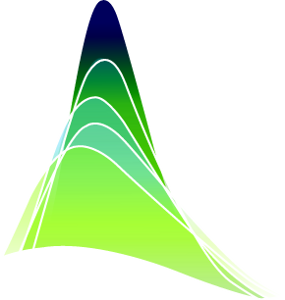
\includegraphics[width=10pc]{ADMB-logo.png}\par
       \vspace{-3.75pc}
      {\large \textcolor{DarkBlue}{\textrm{\textit{\@publisher}}}}\par
     \vskip 1.5em%
%    \end{macrocode}
% We ignore the date.
%    \begin{macrocode}
     % {\large \@date \par}%       % Set date in \large size.
     %\vspace*{1pc}  % Add extra optical space at the bottom.
     \end{center}\par
  \@thanks
  \vfil\null
  \end{titlepage}%
  \setcounter{footnote}{0}%
  \global\let\thanks\relax
  \global\let\maketitle\relax
  \global\let\@thanks\@empty
  \global\let\@author\@empty
  \global\let\@date\@empty
  \global\let\@title\@empty
  \global\let\title\relax
  \global\let\author\relax
  \global\let\date\relax
  \global\let\and\relax
%    \end{macrocode}
% We go to the next page.
%    \begin{macrocode}
  \clearpage
%    \end{macrocode}
% We omit the page number from the next page.
%    \begin{macrocode}
   \thispagestyle{empty}%
%    \end{macrocode}
% If there is a license file, then set it.  If not, leave a blank page.
%    \begin{macrocode}
   \IfFileExists{license.tex}
  {%
    \centerline{\Large License}
    \bigskip
    \InputIfFileExists{license.tex}{}{}
    \vfil\null
  }
  {
  }
  \frontmatter
} % End \maketitle
\fi
%    \end{macrocode}
% \end{macro}
%
% \begin{macro}{\largetitlepart}
%  We want a very large font for the main title.
%    \begin{macrocode}
\newcommand\largetitlepart[1]{%
  %{\sffamily\slshape\bfseries
  {\sffamily\slshape
   \fontsize{36}{36}\selectfont
    #1\par
    \vspace{.5\baselineskip}}%
 }
%    \end{macrocode}
% \end{macro}
%
% \begin{macro}{\mediumtitlepart}
% We also want a title font smaller than the large title one, but not that small.
%    \begin{macrocode}
\newcommand\mediumtitlepart[1]{%
  \medskip
  {%
     \sffamily\slshape
     \fontsize{24}{26}\selectfont
      {#1}\par
    }%
   \bigskip
   \medskip
}
%    \end{macrocode}
% \end{macro}
%
%
% \begin{macro}{\mediumtitlepartnonslanted}
% We want a nonslanted version of |\mediumtitlepart|.
%    \begin{macrocode}
\newcommand\mediumtitlepartnonslanted[1]{%
  \medskip
  {%
     \sffamily
     \fontsize{24}{26}\selectfont
      {#1}\par
    }%
   \bigskip
   \medskip
}
%    \end{macrocode}
% \end{macro}
%
% \begin{macro}{\smalltitlepart}
% We want a yet smaller title font, again still large enough for display (as opposed to text).
%    \begin{macrocode}
\newcommand\smalltitlepart[1]{%
  \medskip
  {%
     \sffamily\slshape
     \fontsize{18}{20}\selectfont
     {#1}\par
   }%
   \bigskip
   \medskip
}
%    \end{macrocode}
% \end{macro}
%
%
% \begin{macro}{\smalltitlepartnonslanted}
% We want a nonslanted version of |\smalltitlepart|
%    \begin{macrocode}
\newcommand\smalltitlepartnonslanted[1]{%
  \smallskip
  {%
     \sffamily
     \fontsize{18}{20}\selectfont
     {#1}\par
   }%
   \bigskip
   \medskip
}
%    \end{macrocode}
% \end{macro}
%
%
% \begin{macro}{\publisher}
% We add a new entity to the title page.
%    \begin{macrocode}
\newcommand*{\publisher}[1]{\gdef\@publisher{#1}}
%    \end{macrocode}
% \end{macro}
%
% We set the publisher to a default value.
%    \begin{macrocode}
\publisher{admb-project.org}
%    \end{macrocode}
%
%
% \subsubsection{Table of Contents}
%
% We want the reference section and the index to show up in the table of contents.  (We still had to do put the index in the \textsc{toc} by hand, though, as we redefine the main index environment.)
%    \begin{macrocode}
% \RequirePackage{tocbibind}
%    \end{macrocode}
%
%
% \begin{macro}{\l@chapter}
%  We want to be able to set math in \textsc{toc} chapter heads, so we add |\boldmath| to the font for the chapter \textsc{toc} entry.
%    \begin{macrocode}
\renewcommand*\l@chapter[2]{%
  \ifnum \c@tocdepth >\m@ne
    \addpenalty{-\@highpenalty}%
    \vskip 1.0em \@plus\p@
    \setlength\@tempdima{1.5em}%
    \begingroup
      \parindent \z@ \rightskip \@pnumwidth
      \parfillskip -\@pnumwidth
%    \end{macrocode}
%  Add the |\boldmath| command here.
%    \begin{macrocode}
      \leavevmode \bfseries \boldmath
      \advance\leftskip\@tempdima
      \hskip -\leftskip
      #1\nobreak\hfil \nobreak\hb@xt@\@pnumwidth{\hss #2}\par
      \penalty\@highpenalty
    \endgroup
  \fi
}
%    \end{macrocode}
% \end{macro}
%
%
% \subsubsection{References}
% 
% We want the reference chapter's name to be ``References'' rather than``Bibliography.''
% 
%    \begin{macrocode}
\renewcommand\tocbibname{References}
%
\let\savebibliography=\bibliography
\renewcommand{\bibliography}{%
   \cleardoublepage
   \pagenumbering[\tocbibname]{bychapter}
   \savebibliography
}
%    \end{macrocode}
%
%
% \subsubsection{The Index}
%
% We want an index.
%    \begin{macrocode}
% \RequirePackage{makeidx}
%    \end{macrocode}
%
% We use this to implement a two-column index where the columns don't crash into each other.
%    \begin{macrocode}
% \RequirePackage{multicol}
%    \end{macrocode}
%
% \begin{macro}{\l@section}
% We need to increase the space for \textsc{toc} number labels (the third argument), that is, for four---not three---numbers and a period.
%    \begin{macrocode}
\renewcommand*\l@section{\@dottedtocline{1}{1.5em}{3em}}
%    \end{macrocode}
% \end{macro}
%
% \begin{macro}{\X}
% An abbreviation for |\index| with one item argument.
%    \begin{macrocode}
\newcommand\X[1]{\index{#1}}   
%    \end{macrocode}
% \end{macro}
%
% \begin{macro}{\XX}
% An abbreviation for |\index| with an item and a sub-item.
%    \begin{macrocode}
\newcommand\XX[2]{\index{#1!#2}}
%    \end{macrocode}
% \end{macro}
%
% \begin{macro}{\fontindexentry}
% \textit{Deprecated, as can only be used with} |\X| and |\XX|.
%    \begin{macrocode}
\newcommand{\fontindexentry}[2]{#2@\csname text#1\endcsname{#2}}
%    \end{macrocode}
% \end{macro}
% 
% \begin{environment}{theindex}
%  We want the index to have two columns that don't crash into each other.\footnote{Modified from Juanjo on LC \LaTeX\ Community.}
%    \begin{macrocode}
\renewenvironment{theindex}
  {\if@twocolumn
      \@restonecolfalse
   \else
      \@restonecoltrue
   \fi
   \setlength{\columnseprule}{0pt}
   \setlength{\columnsep}{45pt}
   \begin{multicols}{2}[\section*{\indexname}]
   %\markboth{\MakeUppercase\indexname}%
    %        {\MakeUppercase\indexname}%
  % \thispagestyle{plain}
  \addcontentsline{toc}{chapter}{\indexname}
   \setlength{\parindent}{0pt}
   \setlength{\parskip}{0pt plus 0.3pt}
   \relax
   \let\item\@idxitem}%
  {\end{multicols}\if@restonecol\onecolumn\else\clearpage\fi}
%
%  We want our special footers for the index pages.
%    \begin{macrocode}
\let\saveprintindex=\printindex
\renewcommand{\printindex}{%
   \cleardoublepage
   \@dopagenumbering
   \pagenumbering[Index]{bychapter}
   \saveprintindex
}
%    \end{macrocode}
% \end{environment}
%
%
% \subsection{Some Document Elements}
%
% \subsubsection{Typesetting Code}
%
% We want so-called ``verbatim'' environments for setting computer code.
%    \begin{macrocode}
% \RequirePackage{fancyvrb}
%    \end{macrocode}
%
% \begin{environment}{code}
% We want the code set a bit smaller than normal size.
%    \begin{macrocode}
\DefineVerbatimEnvironment{code}{Verbatim}{fontsize=\small}
%    \end{macrocode}
% \end{environment}
%
% \begin{environment}{smallcode}
% We want something yet smaller if the above size doesn't fit in the page width.
%    \begin{macrocode}
\DefineVerbatimEnvironment{smallcode}{Verbatim}{fontsize=\scriptsize}
%    \end{macrocode}
% \end{environment}
%
% \begin{environment}{tinycode}
% We want something even smaller yet, in case of dire straits.  This is pretty unreadable.
%    \begin{macrocode}
\DefineVerbatimEnvironment{tinycode}{Verbatim}{fontsize=\tiny}
%    \end{macrocode}
% \end{environment}
%
%
%
% \begin{macro}{\aftercodething}
% We want something that removes extra space above it, and adds extra space below.
%    \begin{macrocode}
\newcommand{\aftercodething}[1]{%
  \unskip
  #1\par
  \medskip
}
%    \end{macrocode}
% \end{macro}
%
%
% We also can use something that formats code more smartly.
%    \begin{macrocode}
% \RequirePackage{listings}
 \lstset{language=C++, numbers=none, basicstyle={\ttfamily}, columns=flexible, showstringspaces=false}
%    \end{macrocode}
%
%
% \begin{macro}{\afterlistingthing}
% We want something that removes extra space above it, and adds extra space below.
%    \begin{macrocode}
\newcommand{\afterlistingthing}[1]{%
  \unskip\vspace{-.5\baselineskip}
  #1\par
  \medskip	
}
%    \end{macrocode}
% \end{macro}
%
%
%
% \subsubsection{Figure and Table Things}
%
% We group together things that might be found in figures and tables, or used with them.
%
%
% \paragraph{Images}
%
% We want to be able to include image files.  They can also be included outside figures/tables.
%    \begin{macrocode}
% \RequirePackage{graphicx}
%    \end{macrocode}
%
% 
% \paragraph{Captions}
%
% We want to be able to have empty captions.
%
%    \begin{macrocode}
% \RequirePackage{caption}
%    \end{macrocode}
%
%
% \begin{macro}{\@setupemptycaption}
% We want a caption that has no following colon.  We use this to implement the command |\emptycaption|.
%    \begin{macrocode}
\newcommand{\@setupemptycaption}{%
  \captionsetup{labelsep=none, justification=centering}
}
%    \end{macrocode}
% \end{macro}
%
% \begin{macro}{\@setupnonemptycaption}
% We also want a caption that does have a following colon.  We use this to implement |\emptycaption|.
%    \begin{macrocode}
\newcommand{\@setupnonemptycaption}{\captionsetup{labelsep=colon}}
%    \end{macrocode}
% \end{macro}
%
% 
% \begin{macro}{\emptycaption}
% We want a command to get an empty caption without a following colon.
%    \begin{macrocode}
\newcommand{\emptycaption}{%
  \@setupemptycaption
  \caption{}
  \@setupnonemptycaption
}
%    \end{macrocode}
% \end{macro}
%
%
% \paragraph{Wrapping around Things}
%
% We want to be able to wrap text around figures or tables.  This is the package (out of this, |floatfiy|, and |picinpar|) that works the best.  |floatflt| doesn't work if two figures come right after another, and |picinpar| doesn't work if the text is shorter than figure.
%    \begin{macrocode}
% \RequirePackage{wrapfig}
%    \end{macrocode}
%
%
% \paragraph{Math Pictures}
%
%  We want to be able to use PicTeX.
%
%  We need |rawfonts| to define, e.g., |\fiverm| for PicTeX, which was written before LaTeX2e.  We have to put it before loading |pictexwd|.
%
%    \begin{macrocode}
% \RequirePackage{rawfonts}
%    \end{macrocode}
%
% \begin{macro}{\@loadrms}
%  We want some more sizes that the package |rawfonts| doesn't define.
%    \begin{macrocode}
\newcommand{\@loadrms}{%
\ifx\undefined\eightrm
  \font\eightrm=cmr8
\fi 
\ifx\undefined\ninerm
  \font\ninerm=cmr9
\fi 
\ifx\undefined\twelverm
  \font\twelverm=cmr12
\fi  
\ifx\undefined\eighteenrm
  \font\eighteenrm=cmr17
\fi 
}
\@loadrms
%    \end{macrocode}
% \end{macro}
%
%    \begin{macrocode}
% \RequirePackage{pictexwd}
%    \end{macrocode}
%  To use |XY|, we need more dimension registers than come with standard LaTeX, so we load |etex|.
%    \begin{macrocode}
% \RequirePackage{etex}
%    \end{macrocode}
%  We want to typeset graphs and diagrams using TeX.
%    \begin{macrocode}
% \RequirePackage{xy}
%    \end{macrocode}
%  
%    \begin{macrocode}
% \RequirePackage{graphics}
%    \end{macrocode}
%  We need color in some of the Pic\TeX\ files.
%    \begin{macrocode}
% \RequirePackage[usenames]{color}
%    \end{macrocode}
%
%
% \subsection{The Finer Tuning}
%
% \subsubsection{Breaking Lines by Hand}
%
% \begin{macro}{\br}
%  We want to be able to force line breaks in, e.g., heads.  This is disabled in contents lines.  Omit the trailing bashslash.
%    \begin{macrocode}
\newcommand{\br}{\hfill\break}
%    \end{macrocode}
% \end{macro}
%
% \begin{macro}{\BR}
%  We want to be able to force line breaks in, e.g., heads.  This stays in force in contents lines.
%    \begin{macrocode}
\newcommand{\BR}{\hfill\break}
%    \end{macrocode}
% \end{macro}
%
% 
% \subsection{Beyond the Traditional Document}
%
% \subsubsection{Hyperlinking}
%
% We want things hyperlinked in the \textsc{pdf}.  This has to be loaded before the |chappg| package!
%    \begin{macrocode}
% \RequirePackage[letterpaper=true,pagebackref=true,linktocpage=true,colorlinks=true]{hyperref}
% \RequirePackage[all]{hypcap}
%    \end{macrocode}
%
%
% \begin{macro}{\addcontentsline}
% We modify the |hyperref| definition, not that of |classes|.
%
% Usage:
%
 % |\addcontentsline{file}{sec_unit}{entry}|, e.g., 
%
% |\addcontentsline{toc}{chapter}{My Chapter Title}|.
%    \begin{macrocode}
\renewcommand\addcontentsline[3]{% toc extension, type, tag
  \begingroup
%    \end{macrocode}
%  We want to ignore the by-hand breaks |\br| in heads, by turning them back into spaces.
%    \begin{macrocode}
    \renewcommand\br{\ }
    \let\label\@gobble
    \ifx\@currentHref\@empty
      \Hy@Warning{%
        No destination for bookmark of \string\addcontentsline,%
        \MessageBreak destination is added%
      }%
      \phantomsection
    \fi
    \expandafter\ifx\csname toclevel@#2\endcsname\relax
      \begingroup
        \def\Hy@tempa{#1}%
        \ifx\Hy@tempa\Hy@bookmarkstype
          \Hy@WarningNoLine{%
            bookmark level for unknown #2 defaults to 0%
          }%
        \else
          \Hy@Info{bookmark level for unknown #2 defaults to 0}%
        \fi
      \endgroup
      \expandafter\gdef\csname toclevel@#2\endcsname{0}%
    \fi
    \edef\Hy@toclevel{\csname toclevel@#2\endcsname}%
    \Hy@writebookmark{\csname the#2\endcsname}%
      {#3}%
      {\@currentHref}%
      {\Hy@toclevel}%
      {#1}%
    \ifHy@verbose
      \def\Hy@tempa{#3}%
      \@onelevel@sanitize\Hy@tempa
      \typeout{pdftex: bookmark at \the\inputlineno: %
        {\csname the#2\endcsname}%
        {\Hy@tempa}%
        {\@currentHref}%
        {\Hy@toclevel}%
        {#1}%
      }%
    \fi
    \addtocontents{#1}{%
      \protect\contentsline{#2}{#3}{\thepage}{\@currentHref}%
    }%
  \endgroup
}
%    \end{macrocode}
% \end{macro}
%
%
% \subsection{Macros to Improve the Look of Things}
% 
% \begin{macro}{\cplus}
% We want the plus signs in ``C++'' to not dominate because of their size.
%    \begin{macrocode}
\newcommand{\cplus}{C\raise.5ex\hbox{\relsize{-3}++}}
%    \end{macrocode}
% \end{macro}
%
% \begin{macro}{\e}
% We want scientific notation to be in the form of ``times 10 exponential'.'
%    \begin{macrocode}
\newcommand{\e}[1]{\ensuremath{\times 10^{#1}}}
%    \end{macrocode}
% \end{macro}
%
%
% \subsubsection{``Assignment By'' Operators}
% 
% We want ``assignment by'' to be spaced well.  Since \LaTeX\ has no notion of these operators, we have to space and kern them by hand.  
%
% \begin{macro}{\pluseq}
% \marg{number variable} |\pluseq| \marg{number variable or number}
%    \begin{macrocode}
\newcommand{\pluseq}{\ensuremath{\:+\kern-.25em=}}
%    \end{macrocode}
% \end{macro}
%
% \begin{macro}{\ttpluseq}
% Like |\pluseq|, but for code mode, not math mode.
%    \begin{macrocode}
\newcommand{\ttpluseq}{{\tt \protect\raisebox{.107ex}{+}=}}
%    \end{macrocode}
% \end{macro}
%
%
% \begin{macro}{\minuseq}
% \marg{number variable} |\minuseq| \marg{number variable or number}
%    \begin{macrocode}
\newcommand{\minuseq}{\ensuremath{\:-\kern-.25em=}}
%    \end{macrocode}
% \end{macro}
%
% \begin{macro}{\ttminuseq}
% Like |\minuseq|, but for code mode, not math mode.
%    \begin{macrocode}
\newcommand{\ttminuseq}{{\tt \protect\raisebox{.273ex}{-}=}}
%    \end{macrocode}
% \end{macro}
%
%
% \begin{macro}{\multiplyeq}
% \marg{number variable} |\multiplyeq| \marg{number variable or number}
%    \begin{macrocode}
\newcommand{\multiplyeq}{\ensuremath{\:*\kern-.22em=}}
%    \end{macrocode}
% \end{macro}
%
% \begin{macro}{\ttmultiplyeq}
% Like |\multiplyeq|, but for code mode, not math mode.
%    \begin{macrocode}
\newcommand{\ttmultiplyeq}{{\tt \protect\raisebox{-.066ex}{*}=}}
%    \end{macrocode}
% \end{macro}
%
%
% \begin{macro}{\divideeq}
% \marg{number variable} |\divideeq| \marg{number variable or number}
%    \begin{macrocode}
\newcommand{\divideeq}{\ensuremath{\:/\kern-.33em=}}
%    \end{macrocode}
% \end{macro}
%
% \begin{macro}{\ttdivideq}
% Like |\divideeq|, but for code mode, not math mode.
%    \begin{macrocode}
\newcommand{\ttdivideeq}{\texttt{/=}}
%    \end{macrocode}
% \end{macro}
%
%
% \subsubsection{Small-Cap Words}
%
% \begin{macro}{\scAB}
% To get \textsc{admb}.
%    \begin{macrocode}

\newcommand{\scAB}{\textsc{admb}}
%    \end{macrocode}
% \end{macro}
%
% \begin{macro}{\scAR}
% To get \textsc{admb-re}.
%    \begin{macrocode}
\newcommand{\scAR}{\mbox{\textsc{admb-re}}}
%    \end{macrocode}
% \end{macro}
%
% \begin{macro}{\scAD}
% To get \textsc{autodif}.
%    \begin{macrocode}
\newcommand{\scAD}{{\textsc{autodif}}}
%    \end{macrocode}
% \end{macro}
%
%
% \subsubsection{Some Abbreviations}
%
% \begin{macro}{\ADM}
%  We don't want everything tied together, as we could get bad line breaks.
%    \begin{macrocode}
\newcommand\ADM{AD~Model Builder}
%    \end{macrocode}
% \end{macro}
%
% \begin{macro}{\ADMS}
%  Same as |\ADM|, but followed by a space.
%    \begin{macrocode}
\newcommand\ADMS{AD~Model Builder }
%    \end{macrocode}
% \end{macro}
%
%    \begin{macrocode}
\makeatother
%    \end{macrocode}
%
% \Finale
\endinput
